%%%%%%%%%%%%%%%%%%%%%%%%%%%%%%%%%%%%%%%%%%%%%%%%%%%%%%%%%%%%%%%%%%%%%%%%%%%%%%%%%%%%%%%
%%%%%%%%%%%%%%%%%%%%%%%%%%%%%%%%%%%%%%%%%%%%%%%%%%%%%%%%%%%%%%%%%%%%%%%%%%%%%%%%%%%%%%%
% 
% This top part of the document is called the 'preamble'.  Modify it with caution!
%
% The real document starts below where it says 'The main document starts here'.

\documentclass[12pt]{article}

\usepackage{amssymb,amsmath,amsthm}
\usepackage[top=1in, bottom=1in, left=1.25in, right=1.25in]{geometry}
\usepackage{fancyhdr}
\usepackage{graphicx}
\usepackage{enumerate}
\usepackage{verbatim}
\usepackage{listings}
\usepackage{xcolor}

% Comment the following line to use TeX's default font of Computer Modern.
\usepackage{times,txfonts}

\definecolor{codegreen}{rgb}{0,0.6,0}
\definecolor{codegray}{rgb}{0.5,0.5,0.5}
\definecolor{codepurple}{rgb}{0.58,0,0.82}
\definecolor{backcolour}{rgb}{0.95,0.95,0.92}

\lstdefinestyle{mystyle}{
    backgroundcolor=\color{backcolour},   
    commentstyle=\color{codegreen},
    keywordstyle=\color{magenta},
    numberstyle=\tiny\color{codegray},
    stringstyle=\color{codepurple},
    basicstyle=\ttfamily\footnotesize,
    breakatwhitespace=false,         
    breaklines=true,                 
    captionpos=b,                    
    keepspaces=true,                 
    numbers=left,                    
    numbersep=5pt,                  
    showspaces=false,                
    showstringspaces=false,
    showtabs=false,                  
    tabsize=2
}

\lstset{style=mystyle}

\newtheoremstyle{homework}% name of the style to be used
  {18pt}% measure of space to leave above the theorem. E.g.: 3pt
  {12pt}% measure of space to leave below the theorem. E.g.: 3pt
  {}% name of font to use in the body of the theorem
  {}% measure of space to indent
  {\bfseries}% name of head font
  {:}% punctuation between head and body
  {2ex}% space after theorem head; " " = normal interword space
  {}% Manually specify head
\theoremstyle{homework} 

% Set up an Exercise environment and a Solution label.
\newtheorem*{exercisecore}{\@currentlabel}
\newenvironment{exercise}[1]
{\def\@currentlabel{#1}\exercisecore}
{\endexercisecore}

\newcommand{\localhead}[1]{\par\smallskip\noindent\textbf{#1}\nobreak\\}%
\newcommand\solution{\localhead{Solution:}}



% \newcommand{includematlab}[1]{\verbatiminput{#1}}

%%%%%%%%%%%%%%%%%%%%%%%%%%%%%%%%%%%%%%%%%%%%%%%%%%%%%%%%%%%%%%%%%%%%%%%%
%
% Stuff for getting the name/document date/title across the header
\makeatletter
\RequirePackage{fancyhdr}
\pagestyle{fancy}
\fancyfoot[C]{\ifnum \value{page} > 1\relax\thepage\fi}
\fancyhead[L]{\ifx\@doclabel\@empty\else\@doclabel\fi}
\fancyhead[C]{\ifx\@docdate\@empty\else\@docdate\fi}
\fancyhead[R]{\ifx\@docauthor\@empty\else\@docauthor\fi}
\headheight 15pt

\def\doclabel#1{\gdef\@doclabel{#1}}
\doclabel{Use {\tt\textbackslash doclabel\{MY LABEL\}}.}
\def\docdate#1{\gdef\@docdate{#1}}
\docdate{Use {\tt\textbackslash docdate\{MY DATE\}}.}
\def\docauthor#1{\gdef\@docauthor{#1}}
\docauthor{Use {\tt\textbackslash docauthor\{MY NAME\}}.}
\makeatother

%% General formatting parameters
\parindent 0pt
\parskip 12pt plus 1pt

\def\vx{\mathbf x}
\def\vb{\mathbf b}

% Shortcuts for blackboard bold number sets (reals, integers, etc.)
\newcommand{\Reals}{\ensuremath{\mathbb R}}
\newcommand{\Nats}{\ensuremath{\mathbb N}}
\newcommand{\Ints}{\ensuremath{\mathbb Z}}
\newcommand{\Rats}{\ensuremath{\mathbb Q}}
\newcommand{\Cplx}{\ensuremath{\mathbb C}}
%% Some equivalents that some people may prefer.
\let\RR\Reals
\let\NN\Nats
\let\II\Ints
\let\CC\Cplx

%%%%%%%%%%%%%%%%%%%%%%%%%%%%%%%%%%%%%%%%%%%%%%%%%%%%%%%%%%%%%%%%%%%%%%%%%%%%%%%%%%%%%%%
%%%%%%%%%%%%%%%%%%%%%%%%%%%%%%%%%%%%%%%%%%%%%%%%%%%%%%%%%%%%%%%%%%%%%%%%%%%%%%%%%%%%%%%
% 
% The main document start here.

% The following commands set up the material that appears in the header.

%%%%%%%%%%%%%%%%%%%%%%%%%%%%%%%%%%%%%%%%%%%%%%%%%%%%%%%%%%%%%%%%%%%%%%%%%%
\doclabel{Math 426: Homework 10}
\docauthor{Andrew Player}
\docdate{November 4, 2020}

\begin{document}

\begin{exercise}{Supplemental 1}
Consider these three points: $\{(1, 1), (2.5, 8), (4, 5)\}$.
Find the polynomial $P(x)$ of degree 2 which passes through these points. Do this three different ways, by using
\begin{enumerate}
\item[(a)] the Vandermonde matrix method,
\item[(b)] the Newton form and its triangular matrix method, and
\item[(c)] the Lagrange form.
\end{enumerate}
\end{exercise}
a.)\newline
\begin{lstlisting}
% Vandermonde Method
>> V = [1 1 1; 1 2.5 2.5^2; 1 4 16];
>> b = [1 8 5];
>> V/b

ans =

   0.155555555555556
   0.580555555555556
   1.255555555555556
\end{lstlisting}
b.)\newline
\begin{bmatrix}
1 & 0 & 0\\
8 & 14/3 & 0\\
5 & -2 & -20/9
\end{bmatrix}
\begin{equation}
f(x) = 1 + \frac{14}{3}(x-1) + \frac{-20}{9}(x-1)(x-2.5)
\end{equation}
c.)
\begin{equation}
(1)\frac{(x-2.5)(x-4)}{(1-2.5)(1-4)} + (8)\frac{(x-1)(x-4)}{(2.5-1)(2.5-4)} + (5)\frac{(x-1)(x-2.5)}{(4-1)(4-2.5)}
\end{equation} 

\begin{exercise}{Supplemental 2}
Consider the $x$ coordinates $x_0=0$, $x_1=\pi/3$, $x_2=2\pi/3$ and $x_3=\pi$.
\begin{enumerate}
	\item[a)] Plot the four Lagrange basis functions $\phi_k$ $k=0,\ldots,4$ on a single graph with domain $[0,\pi]$.
	\item[b)] Plot the four Newton interpolation basis functions
	$\psi_k$, each on its own individual graph.
	\item[c)] Plot the graph of $\sin(x)$ along with its Lagrange interpolant $p_{\mathrm{Lag}}$.
	\item[d)] Plot the graph of $\sin(x)$ along with its Newton interpolant $p_{\mathrm{Newt}}$.
	\item[e)] What is the relative error of $p_{\mathrm{Lag}}(\pi/4)$?
\end{enumerate}
\end{exercise}
a.)\newline
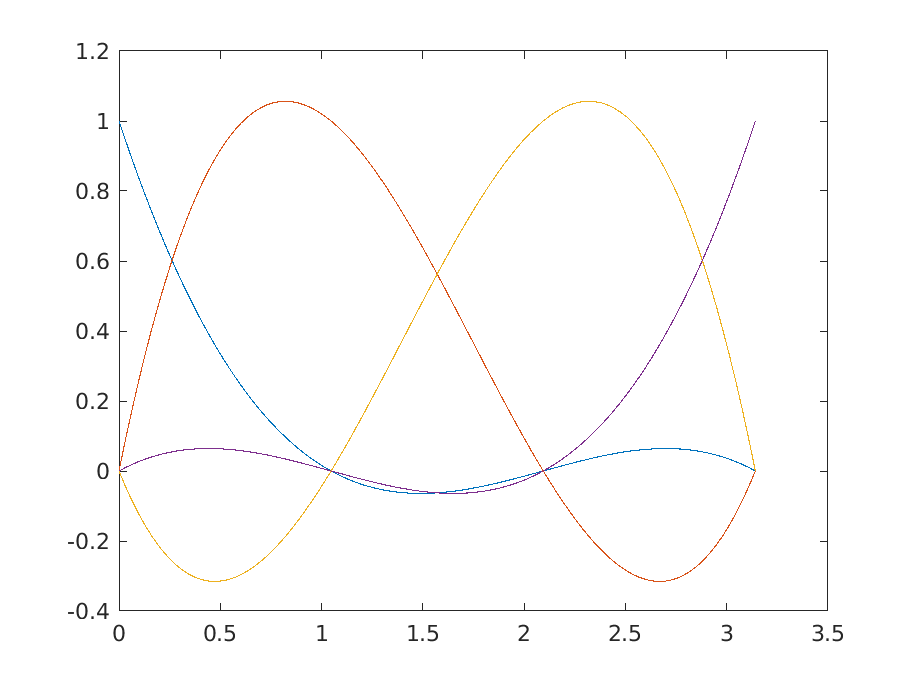
\includegraphics[scale=0.45]{lagbasisplots.png}\newline
b.)\newline
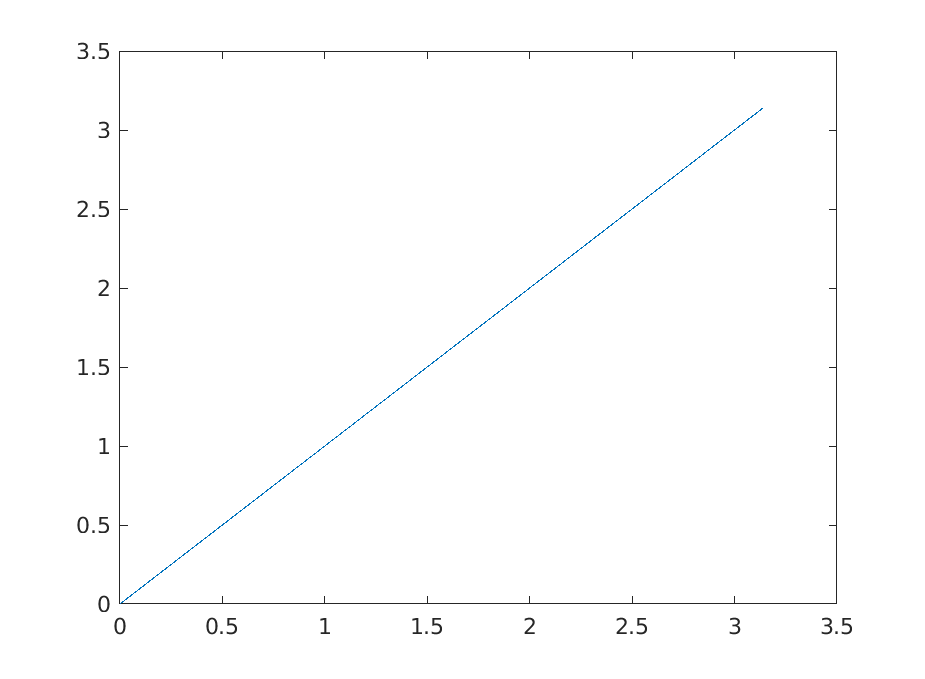
\includegraphics[scale=0.45]{n1.png}\newline
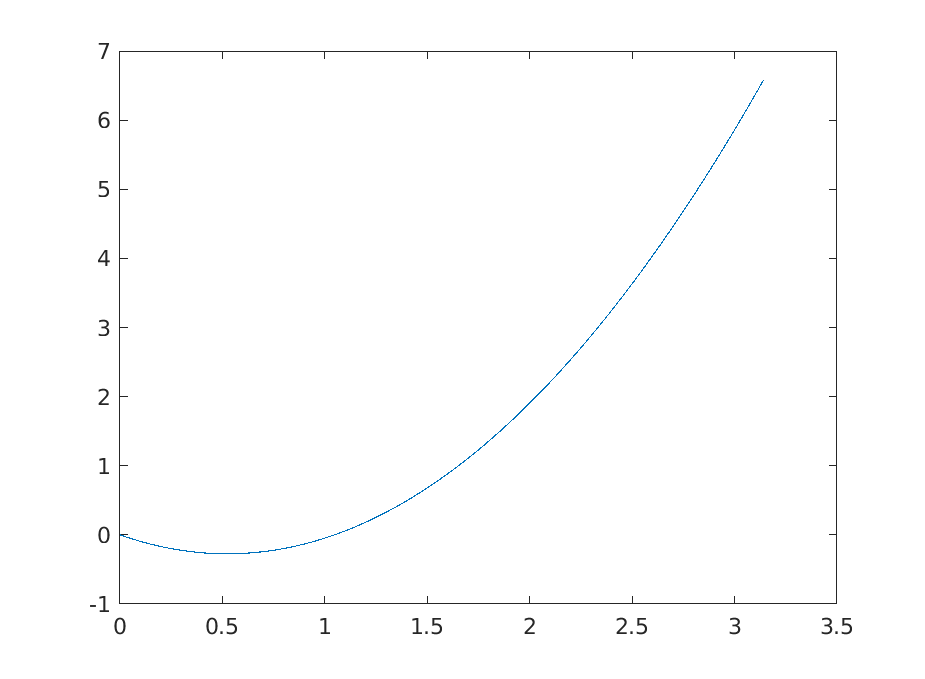
\includegraphics[scale=0.45]{n2.png}\newline
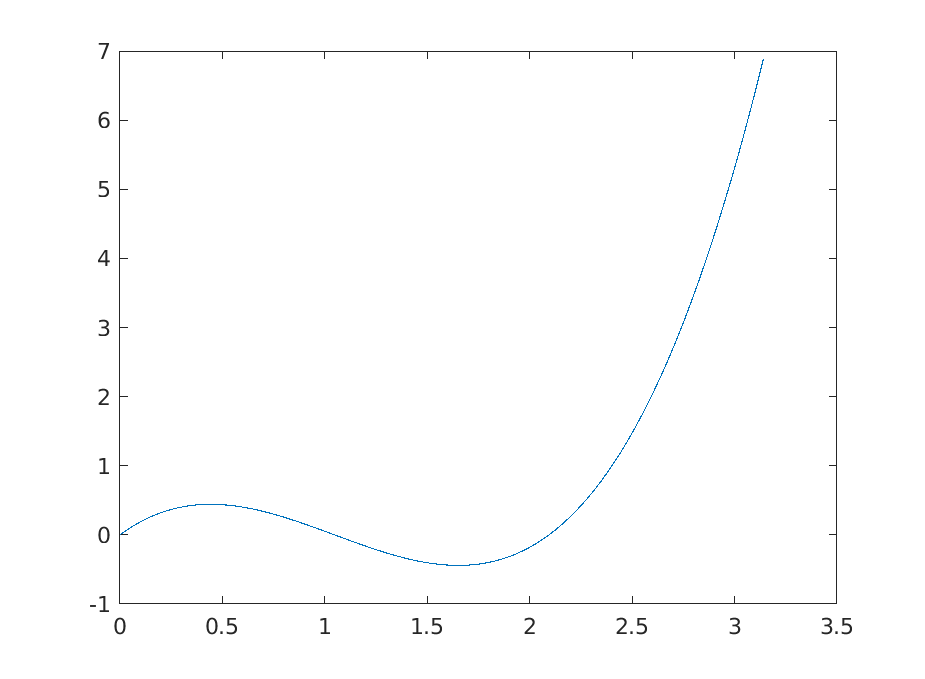
\includegraphics[scale=0.45]{n3.png}\newline
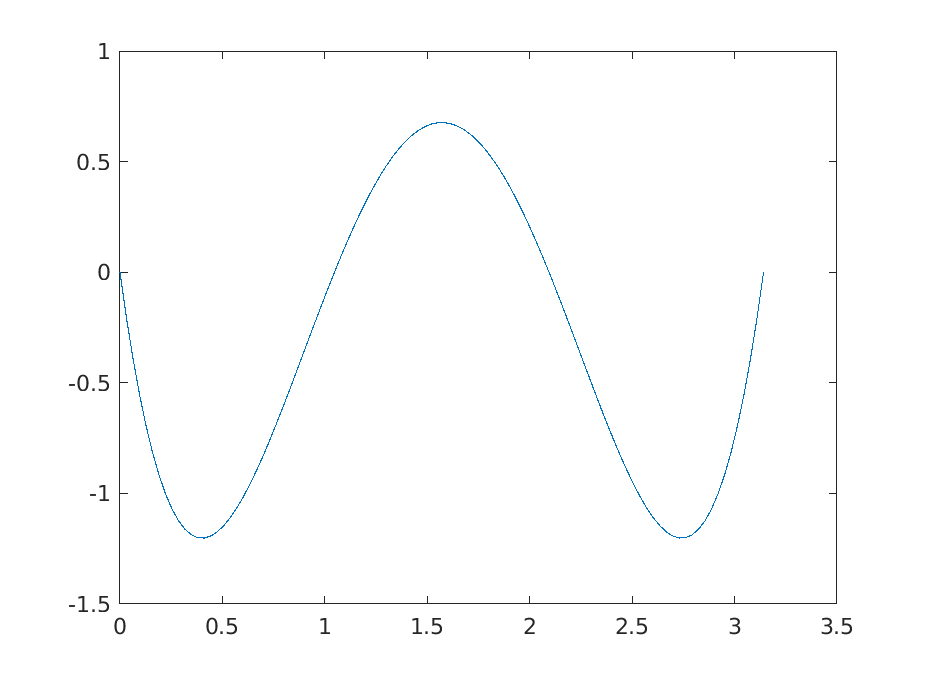
\includegraphics[scale=0.45]{n4.png}\newline
c.)\newline
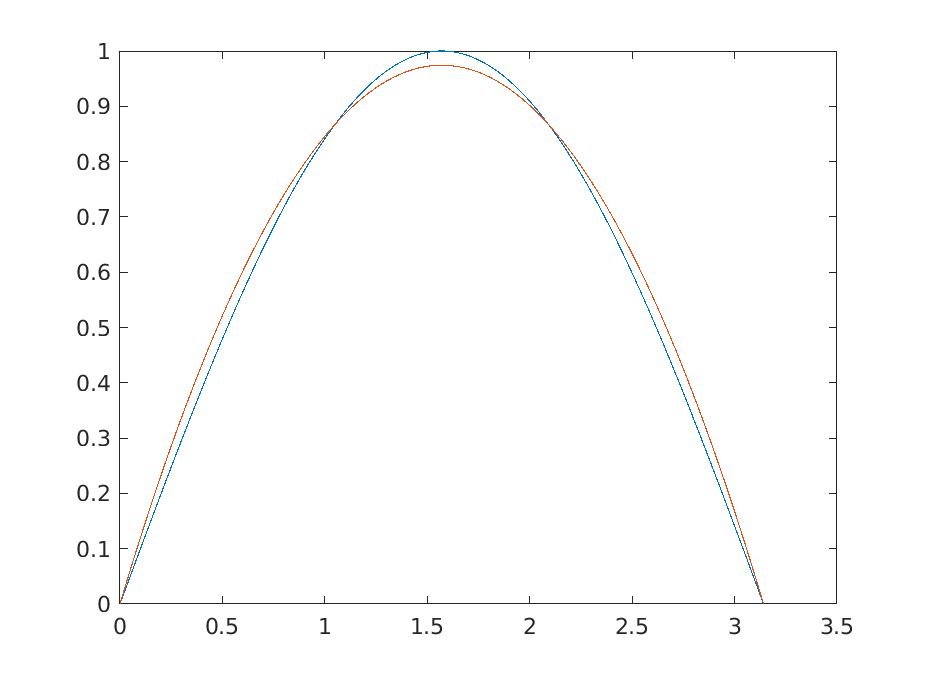
\includegraphics[scale=0.45]{sinelagbetter.png}\newline
d.)\newline
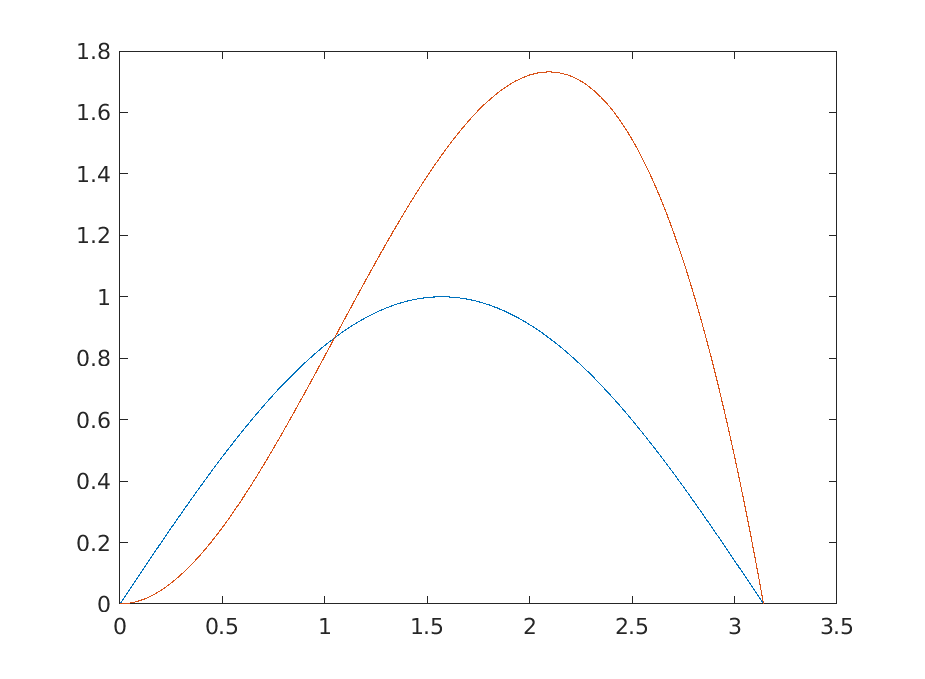
\includegraphics[scale=0.45]{sinelag.png}\newline
e.)\newline


\begin{exercise}{Exercise 8.1}
\end{exercise}
a.)\newline
\begin{lstlisting} [language = Matlab]
  >> years = [1900 1920 1940 1960 1980 2000];
  >> pop = [76 105.7 131.7 179.3 226.5 281.4];
  >> P = polyfit(years, pop, 5);
  >> x = [1900:1:2020];
  >> y = polyval(P, x);
  >> y(121) % Population in 2020
  ans = 
       4.595999755859375e+02
\end{lstlisting}
Plots:\newline
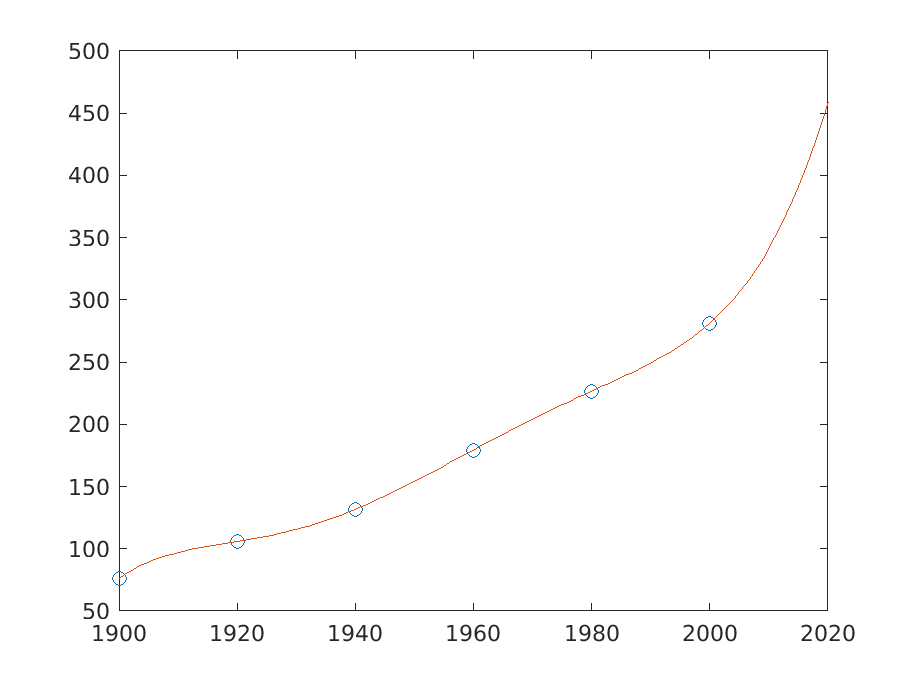
\includegraphics[scale=0.45]{polypopplot.png}\newline
b.)\newline
\begin{equation}
(79)\frac{(x-1920)(x-1940)}{(1900-1920)(1900-1940)}+(105.7)\frac{(x-1900)(x-1940)}{(1920-1900)(1920-1940)}+(131.7)\frac{(x-1900)(x-1920)}{(1940-1900)(1940-1920)}
\end{equation}
c.)\newline
0th: $76$\newline
1st: $0.6734006$\newline
2nd: $0.00239575$\newline
Polynomial: $76 + 0.6734006(x-1900) + 0.00239575(x-1900)(x-1920)$\newline


\begin{exercise}{Exercise 8.2}
\end{exercise}
Formula is $3x^2+-2x-2$ from
\begin{lstlisting}[language = Matlab]
  >> polyfit(xs, ys, 2);
  >> P = polyfit(xs, ys, 2);
  >> P

    P =

      2.999999999999999  -1.999999999999999  -2.000000000000000
\end{lstlisting}
So, $x_3 = 1.2152504370215301$

\begin{exercise}{Midterm, problem 6}
\end{exercise}
a.)\newline
Let $f$ be $C^{n+1}$ on $(a, x)$, where $a, x\ \epsilon\ R$. Then
\begin{equation}
f(x) = f(a)+f'(a)(x-a)+\frac{f''(a)}{2!}(x-a)^2+...+\frac{f^{n}(a)}{n!}(x-a)^{n}+R_n(x)
\end{equation}
where 
\begin{equation}
R_n(x) = \frac{f^{n+1}(c)}{(n+1)!}(x-a)^{n+1}
\end{equation}
for some $c\ \epsilon\ R$ between $a$ and $x$.
\newline
b.)\newline
\begin{equation}
sin(x) = sin(0) + 2cos(0)(x-0) + \frac{-4sin(0)}{2!}(x-0)^2 + \frac{-8cos(0)}{3!}(x-0)^3
\end{equation}
\begin{equation}
       = 2x + \frac{-4}{3}x^3
\end{equation}
c.)\newline
$R_n(x) = \frac{f^{4}(c)}{(4)!}(x-a)^{4}$\newline
$f^{4}(c)} <= max(f^{4}(x))$\newline
$e^c <= max(e^x)$ on $0 <= x <= 2$\newline
So, c = 2, and:\newline
Max Error $= \frac{e^{2}}{24}2^4 = 9*16/24 = 6$

\end{document}